% Options for packages loaded elsewhere
\PassOptionsToPackage{unicode}{hyperref}
\PassOptionsToPackage{hyphens}{url}
%
\documentclass[
]{article}
\usepackage{amsmath,amssymb}
\usepackage{lmodern}
\usepackage{iftex}
\ifPDFTeX
  \usepackage[T1]{fontenc}
  \usepackage[utf8]{inputenc}
  \usepackage{textcomp} % provide euro and other symbols
\else % if luatex or xetex
  \usepackage{unicode-math}
  \defaultfontfeatures{Scale=MatchLowercase}
  \defaultfontfeatures[\rmfamily]{Ligatures=TeX,Scale=1}
\fi
% Use upquote if available, for straight quotes in verbatim environments
\IfFileExists{upquote.sty}{\usepackage{upquote}}{}
\IfFileExists{microtype.sty}{% use microtype if available
  \usepackage[]{microtype}
  \UseMicrotypeSet[protrusion]{basicmath} % disable protrusion for tt fonts
}{}
\makeatletter
\@ifundefined{KOMAClassName}{% if non-KOMA class
  \IfFileExists{parskip.sty}{%
    \usepackage{parskip}
  }{% else
    \setlength{\parindent}{0pt}
    \setlength{\parskip}{6pt plus 2pt minus 1pt}}
}{% if KOMA class
  \KOMAoptions{parskip=half}}
\makeatother
\usepackage{xcolor}
\IfFileExists{xurl.sty}{\usepackage{xurl}}{} % add URL line breaks if available
\IfFileExists{bookmark.sty}{\usepackage{bookmark}}{\usepackage{hyperref}}
\hypersetup{
  pdftitle={COVID-19 Forecast Similarity Analysis},
  pdfauthor={Nutcha Wattanachit, Johannes Bracher, Evan Ray, Nick Reich},
  hidelinks,
  pdfcreator={LaTeX via pandoc}}
\urlstyle{same} % disable monospaced font for URLs
\usepackage[margin=1in]{geometry}
\usepackage{graphicx}
\makeatletter
\def\maxwidth{\ifdim\Gin@nat@width>\linewidth\linewidth\else\Gin@nat@width\fi}
\def\maxheight{\ifdim\Gin@nat@height>\textheight\textheight\else\Gin@nat@height\fi}
\makeatother
% Scale images if necessary, so that they will not overflow the page
% margins by default, and it is still possible to overwrite the defaults
% using explicit options in \includegraphics[width, height, ...]{}
\setkeys{Gin}{width=\maxwidth,height=\maxheight,keepaspectratio}
% Set default figure placement to htbp
\makeatletter
\def\fps@figure{htbp}
\makeatother
\setlength{\emergencystretch}{3em} % prevent overfull lines
\providecommand{\tightlist}{%
  \setlength{\itemsep}{0pt}\setlength{\parskip}{0pt}}
\setcounter{secnumdepth}{-\maxdimen} % remove section numbering
\usepackage{tabularx}
\usepackage{hyperref}
\usepackage{wrapfig}
\usepackage{float}
\usepackage{colortbl}
\usepackage{pdflscape}
\usepackage{tabu}
\usepackage{xcolor}
\ifLuaTeX
  \usepackage{selnolig}  % disable illegal ligatures
\fi

\title{COVID-19 Forecast Similarity Analysis}
\author{Nutcha Wattanachit, Johannes Bracher, Evan Ray, Nick Reich}
\date{10/10/2022}

\begin{document}
\maketitle

\hypertarget{concept-examples-of-forecasts-and-cramer-distances---ca}{%
\section{Concept: Examples of forecasts and Cramer distances -
CA}\label{concept-examples-of-forecasts-and-cramer-distances---ca}}

The plots show the distances between the ensemble and UMass-MechBayes at
two different forecast dates. We can see that lower approximated CD
values indicates more similarity between the two forecasts - as the
plots of the predictive quantiles on forecast date 2021-04-05 shows a
lot of overlap. On the other hand, the plots of the predictive quantiles
on forecast date 2021-08-02 shows less overlap accompanying by higher
approximated CD values.

\begin{figure}

{\centering 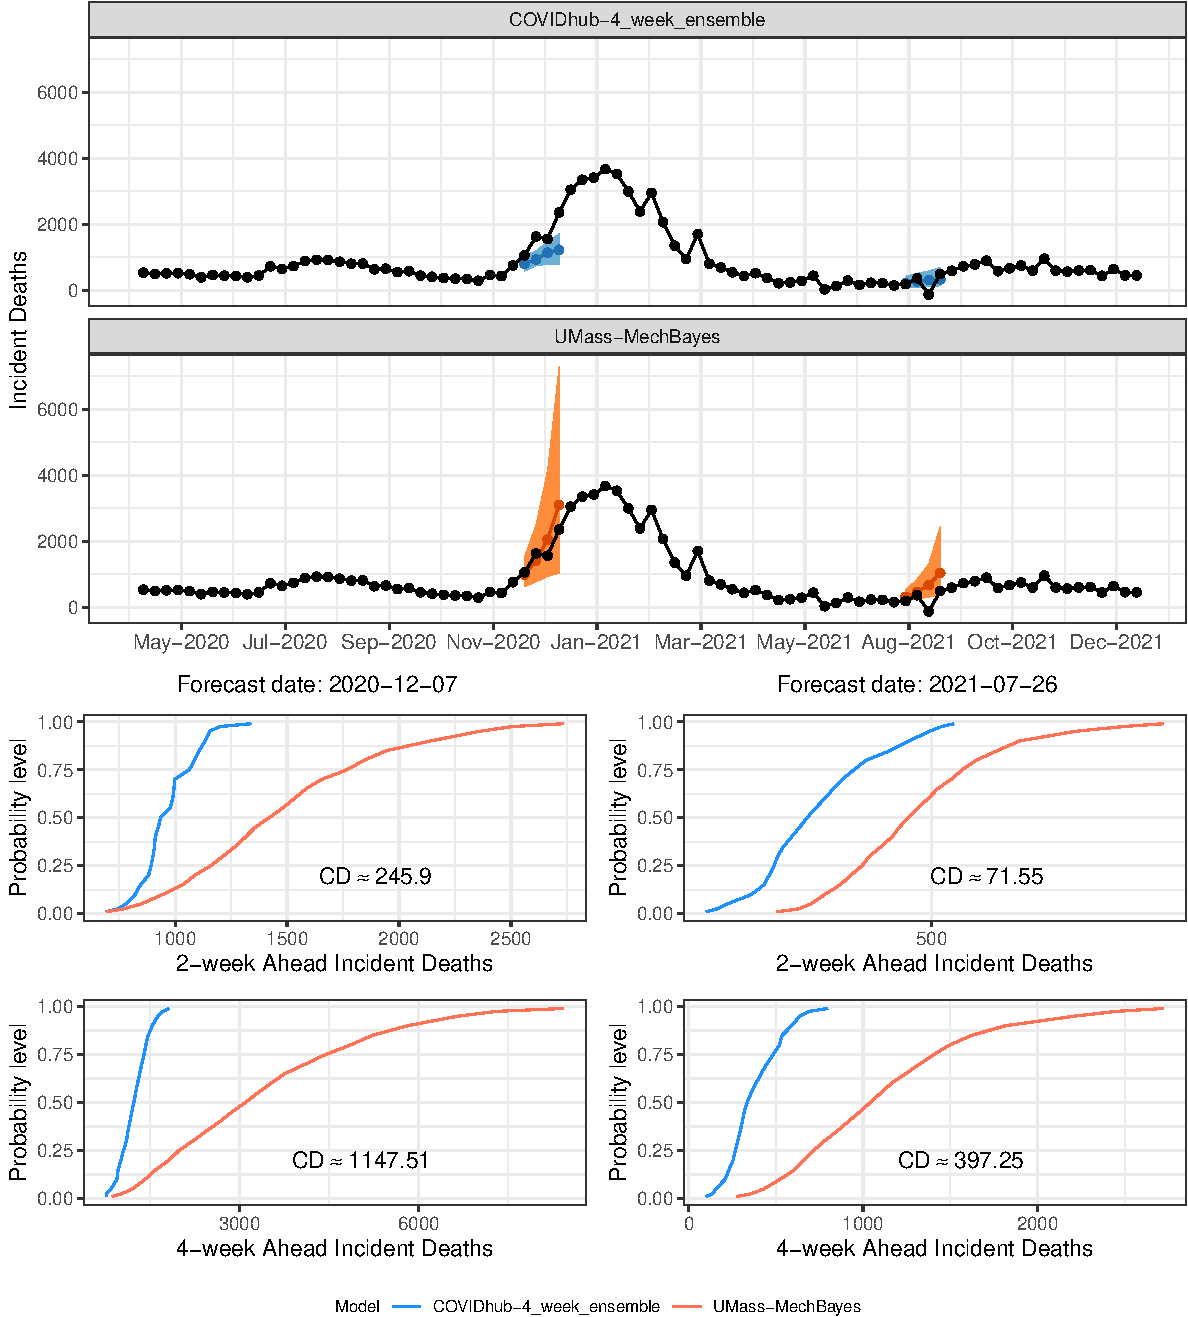
\includegraphics{sim_analysis_4_files/figure-latex/concept_ca-1} 

}

\caption{COVID-19 deaths forecasts (left) and all predictive quantiles (right)}\label{fig:concept_ca}
\end{figure}

\hypertarget{overall-similarities}{%
\subsection{Overall Similarities}\label{overall-similarities}}

\begin{itemize}
\tightlist
\item
  Targets: all wk ahead inc deaths
\item
  End dates: May 02 2020-Dec 18 2021
\item
  Model: The same set as in the evaluation paper (28 models) that have 4
  horizons on each submission and that have more than 10000k submissions
\item
  Probability levels: All
\item
  Locations: National and states (excluding US territory and DC), so 51
  locations
\end{itemize}

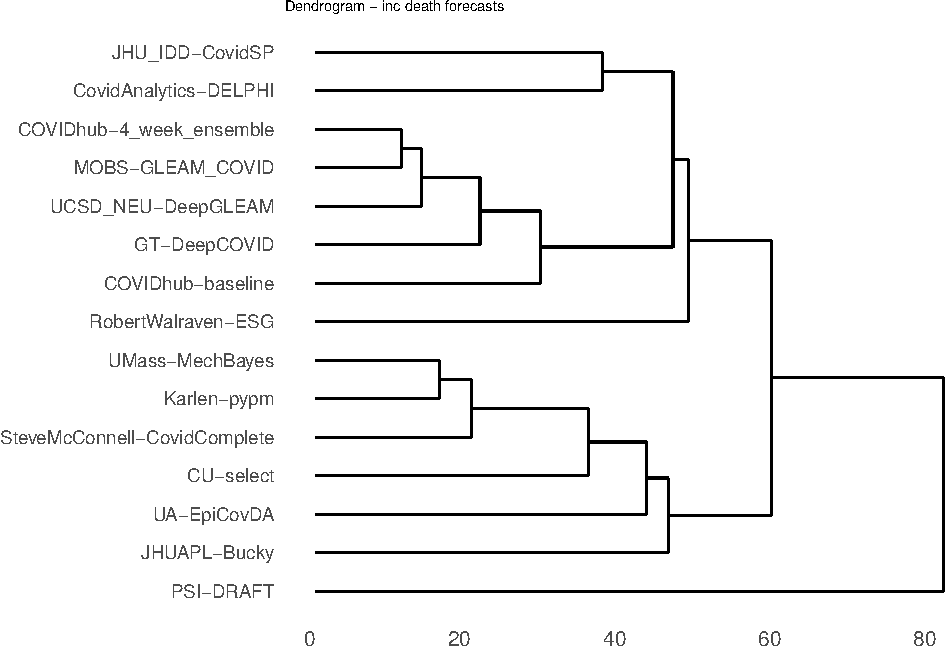
\includegraphics{sim_analysis_4_files/figure-latex/dendro-1.pdf}

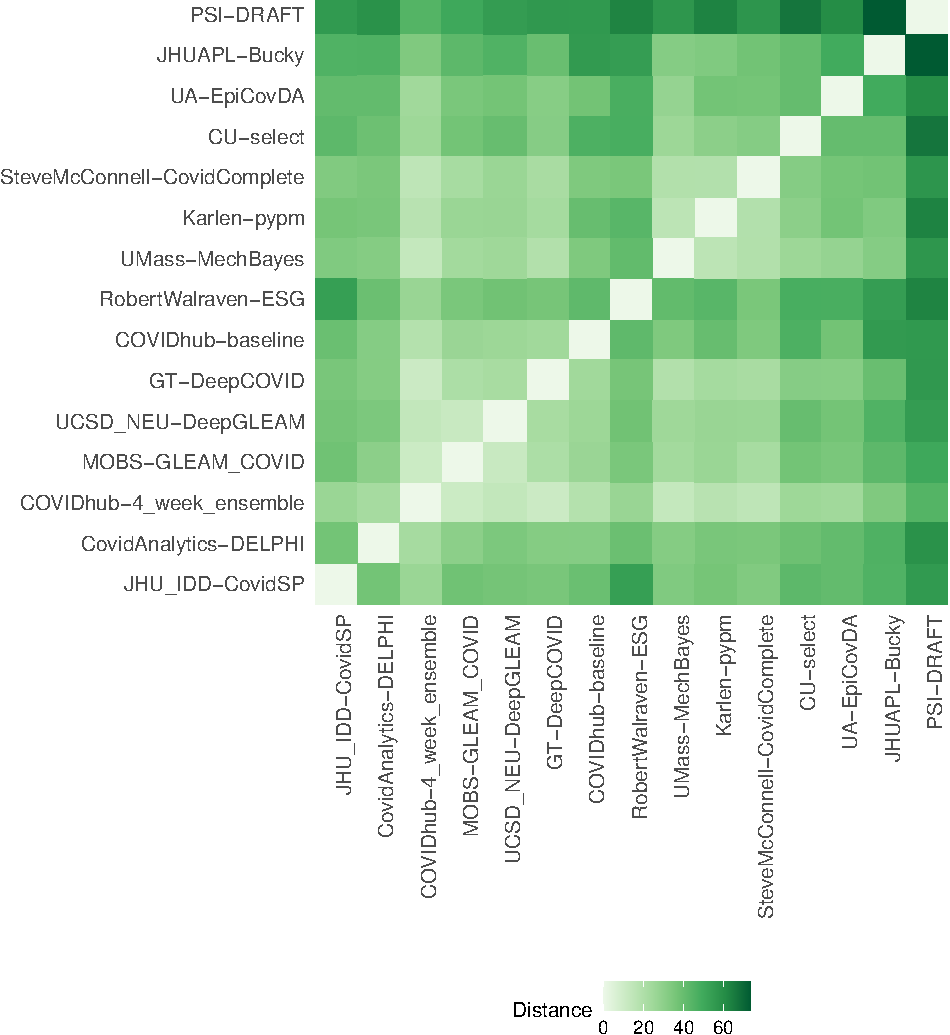
\includegraphics{sim_analysis_4_files/figure-latex/unnamed-chunk-3-1.pdf}

\hypertarget{distancedissimilarity-as-a-signalleading-indicator-of-an-increase-in-incident-deaths}{%
\section{Distance/dissimilarity as a signal/leading indicator of an
increase in incident
deaths}\label{distancedissimilarity-as-a-signalleading-indicator-of-an-increase-in-incident-deaths}}

Cross-correlations of median approx. CDs and incident deaths are
calculated for 2 ``up'' periods, the winter 2020 and the fall 2021, are
calculated for 34 selected states based on the criteria below. The
maximum lags and leads are 9 weeks before and after each target dates
during 9 weeks of up periods.

\hypertarget{forecast-inclusion-criteria}{%
\subsection{Forecast inclusion
criteria}\label{forecast-inclusion-criteria}}

\begin{itemize}
\tightlist
\item
  Targets: 2 and 4 wk ahead inc death
\item
  Target End Dates: Jan 2021-Jan 2022
\item
  Model: all models submitted on a particular date
\item
  Probability levels: All
\item
  Locations: All 34 states (continental US) except HI, AK and DC. We
  also exclude DE, ME,MT,OK,OR,VT for low or highly variable incidents.
  We also exclude AZ, CA, CT, MD, MO, NE, NJ, RI since they have only
  one peak.
\end{itemize}

\hypertarget{cross-correlations}{%
\subsection{Cross correlations}\label{cross-correlations}}

The distributions of cross-correlations across the two up periods of
winter 2020/2021 and fall 2021 waves (and 9 weeks before the first week
and 9 after the last week) show that there is no evidence that the
median CDs of 2 week ahead forecasts consistently lead or lag the
increase in incident deaths, however there is some evidence that the
median CDs of 4 week ahead forecasts lead the increase in incident
deaths.

\begin{figure}

{\centering 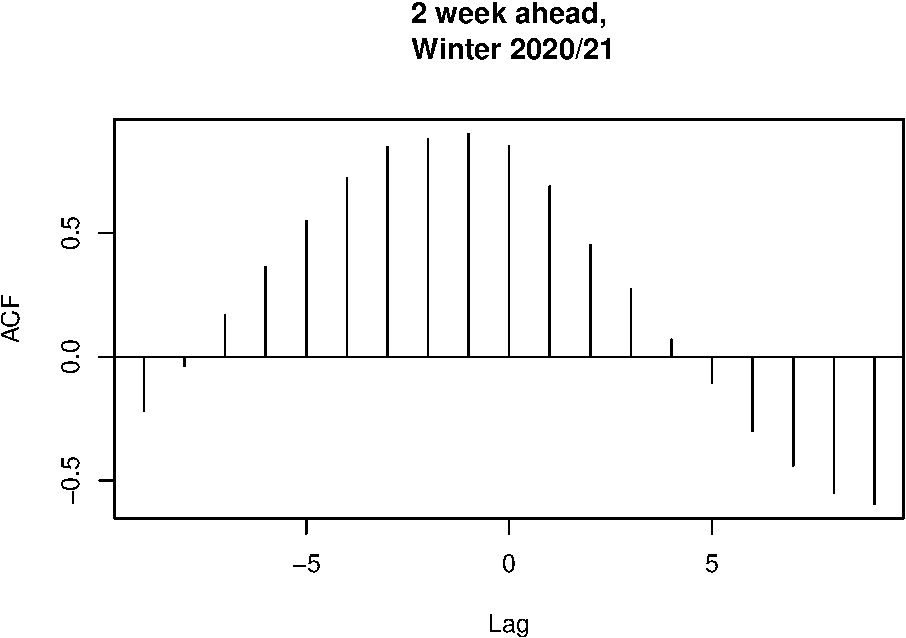
\includegraphics[width=1\linewidth,height=1\textheight]{sim_analysis_4_files/figure-latex/corex-1} 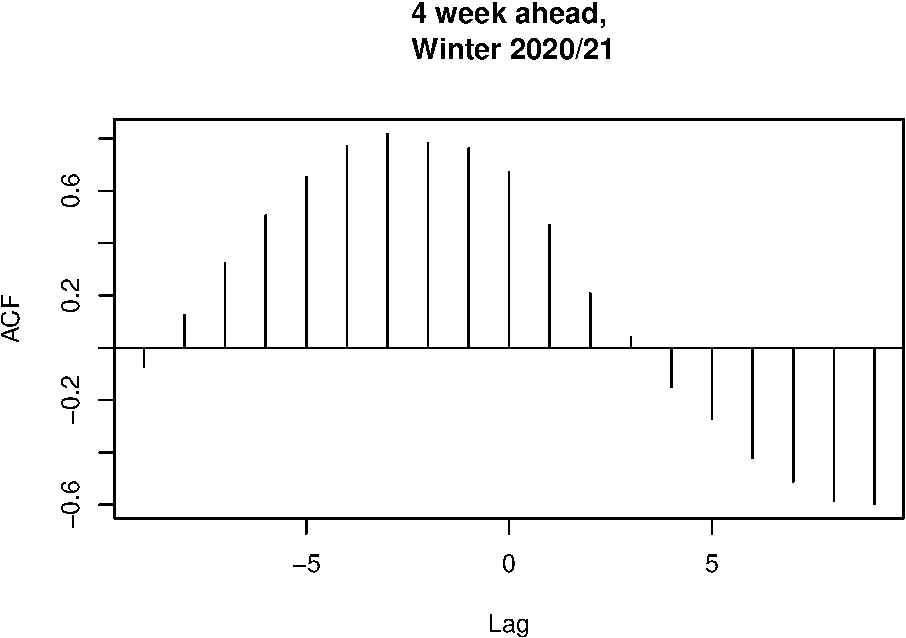
\includegraphics[width=1\linewidth,height=1\textheight]{sim_analysis_4_files/figure-latex/corex-2} 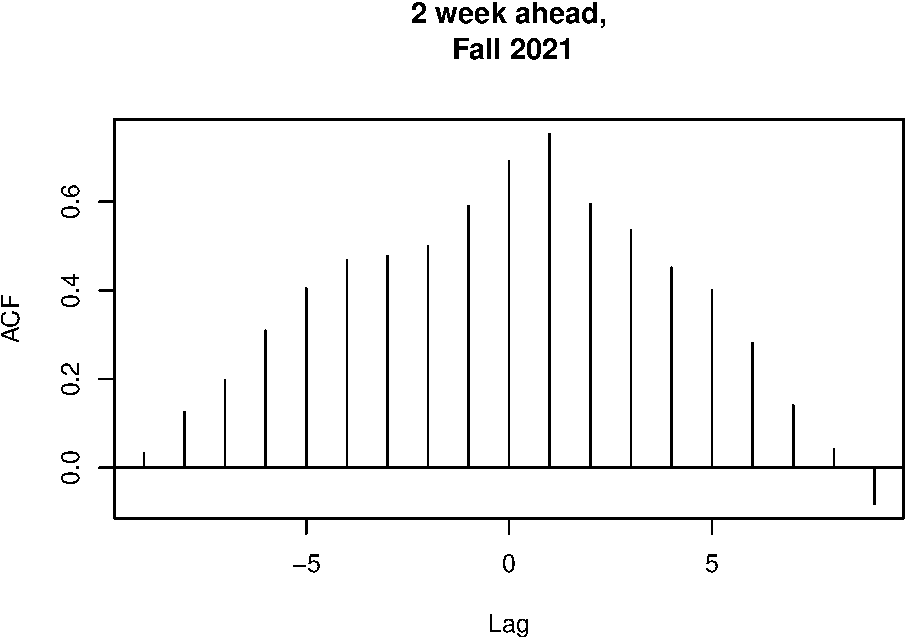
\includegraphics[width=1\linewidth,height=1\textheight]{sim_analysis_4_files/figure-latex/corex-3} 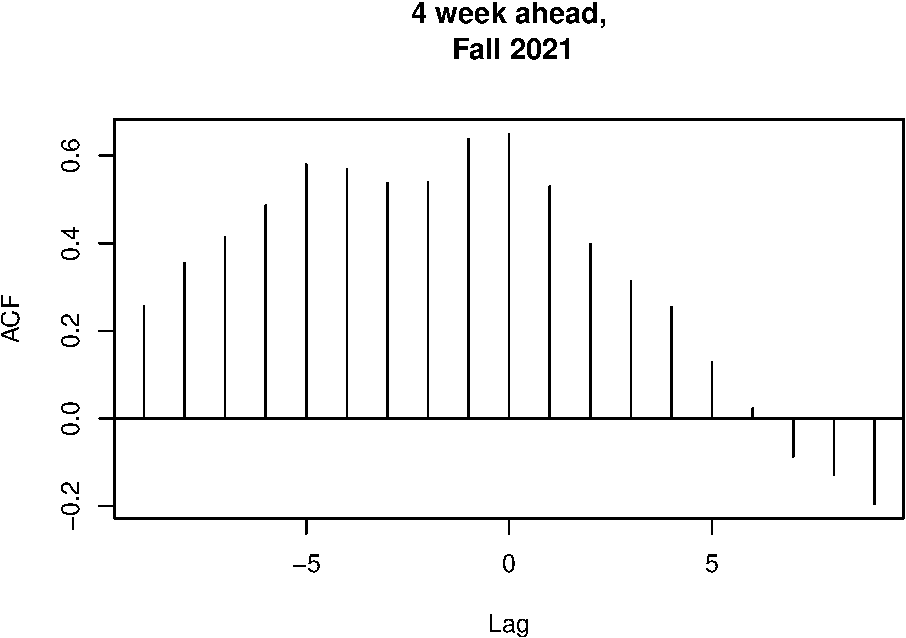
\includegraphics[width=1\linewidth,height=1\textheight]{sim_analysis_4_files/figure-latex/corex-4} 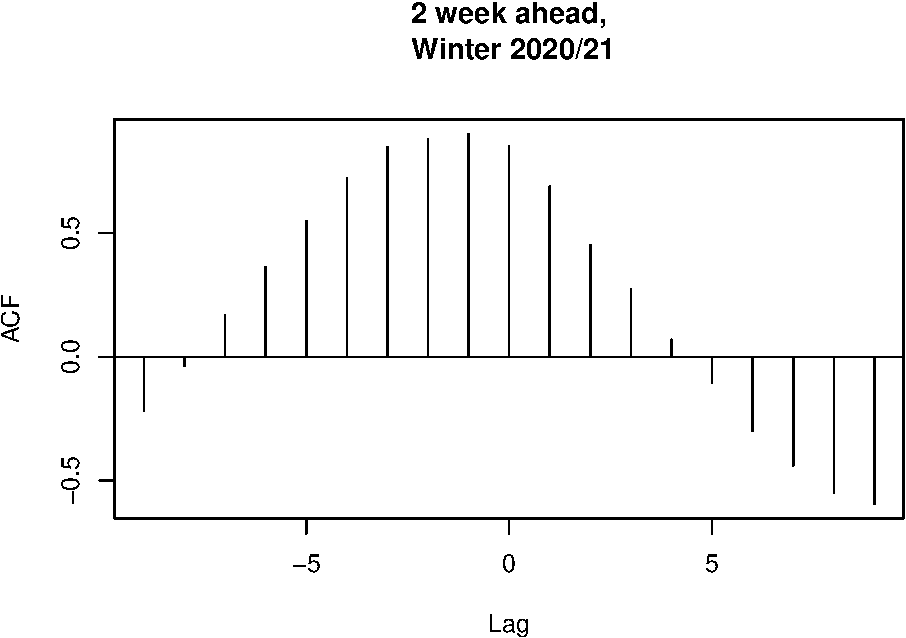
\includegraphics[width=1\linewidth,height=1\textheight]{sim_analysis_4_files/figure-latex/corex-5} 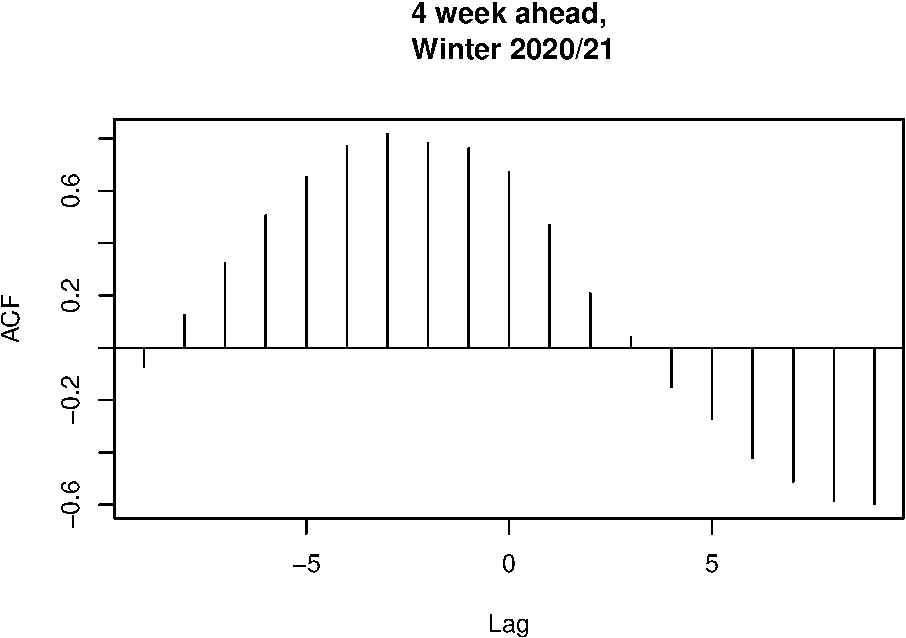
\includegraphics[width=1\linewidth,height=1\textheight]{sim_analysis_4_files/figure-latex/corex-6} 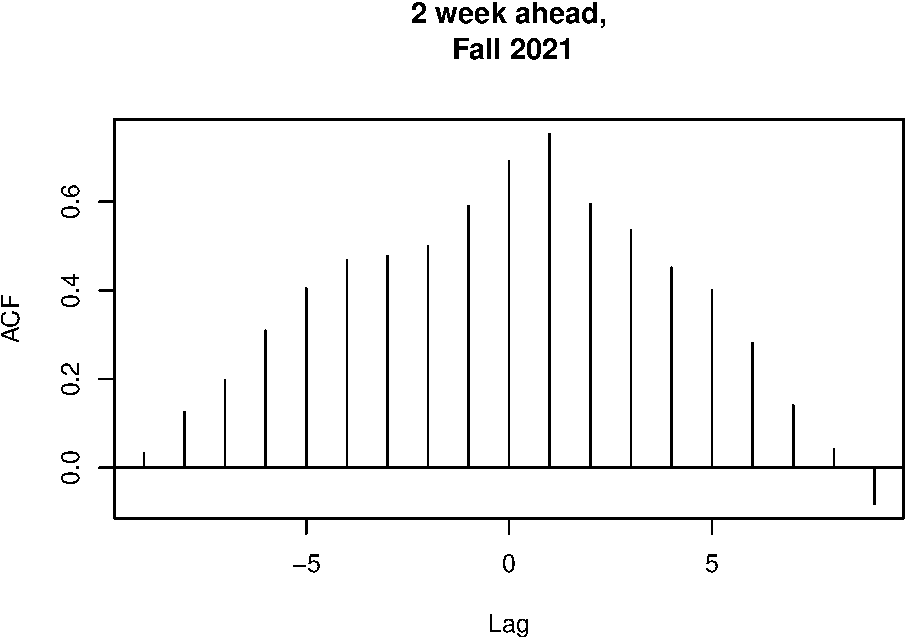
\includegraphics[width=1\linewidth,height=1\textheight]{sim_analysis_4_files/figure-latex/corex-7} 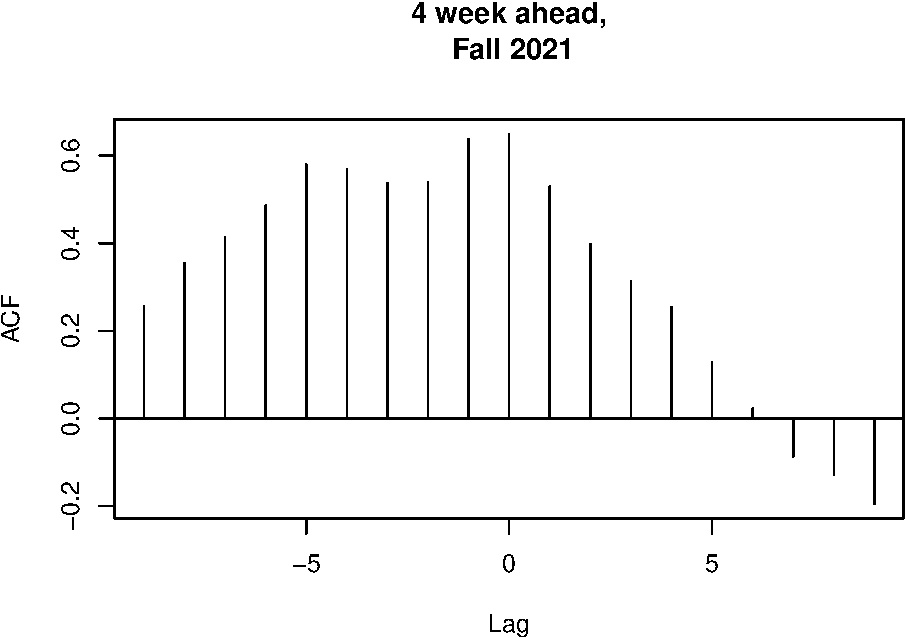
\includegraphics[width=1\linewidth,height=1\textheight]{sim_analysis_4_files/figure-latex/corex-8} 

}

\caption{Example CCF plots for 2 and 4 wk ahead horizons.}\label{fig:corex}
\end{figure}

\begin{figure}

{\centering 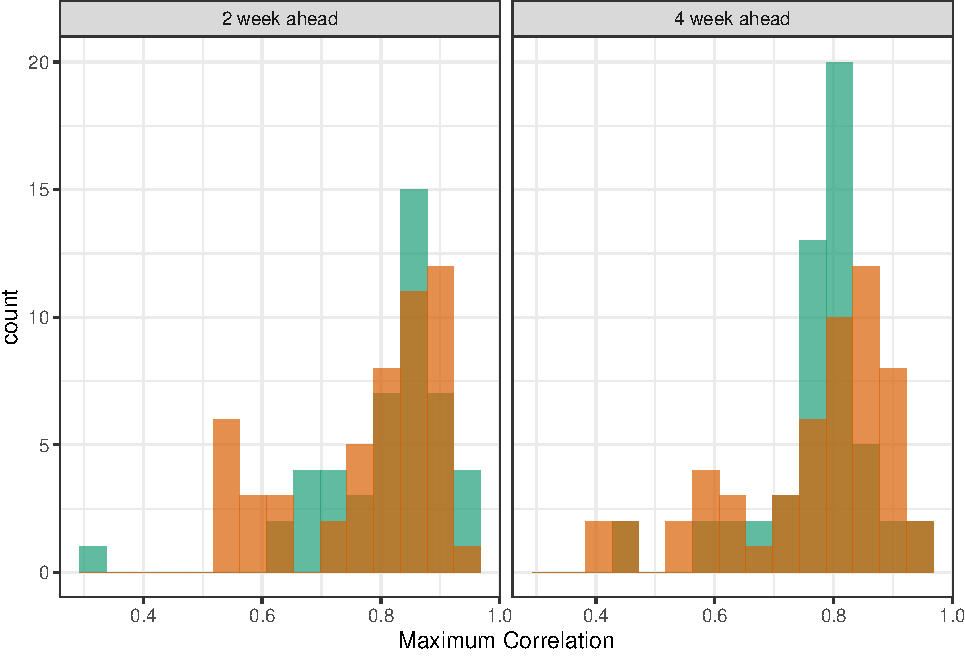
\includegraphics[width=1\linewidth,height=1\textheight]{sim_analysis_4_files/figure-latex/corm1-1} 

}

\caption{Distribution of max. correlations by horizon and time}\label{fig:corm1}
\end{figure}

\begin{figure}

{\centering 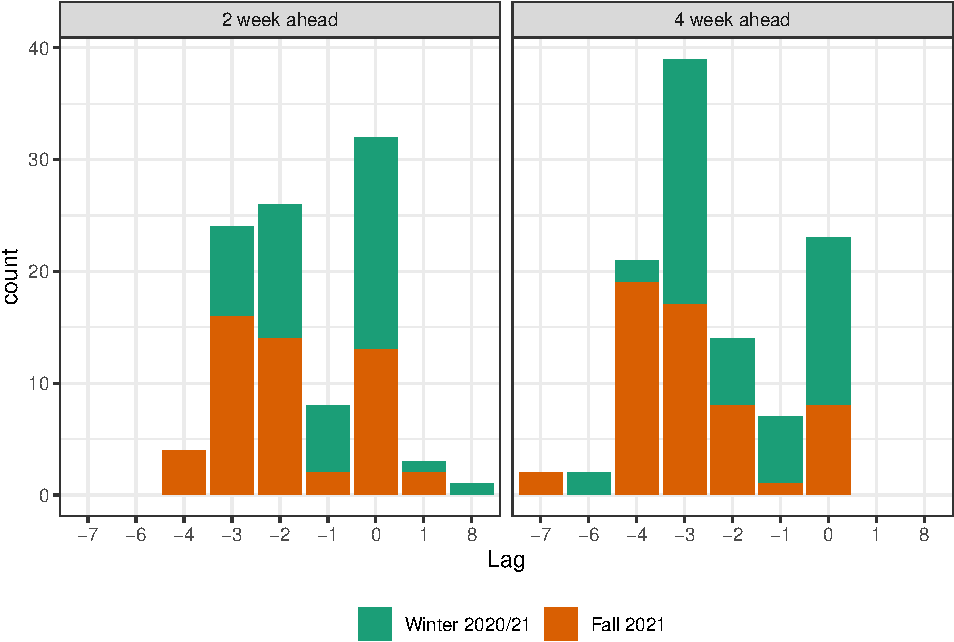
\includegraphics[width=1\linewidth,height=1\textheight]{sim_analysis_4_files/figure-latex/corm2-1} 

}

\caption{Count of lags of max. cross-correlations}\label{fig:corm2}
\end{figure}

\end{document}
